\documentclass[t]{beamer}
\mode<presentation>

\usepackage{etex}

\usetheme{Madrid}
% other themes: Warsaw, AnnArbor, Antibes, Bergen, Berkeley, Berlin, Boadilla, boxes, CambridgeUS, Copenhagen, Darmstadt, default, Dresden, Frankfurt, Goettingen,
% Hannover, Ilmenau, JuanLesPins, Luebeck, Madrid, Maloe, Marburg, Montpellier, PaloAlto, Pittsburg, Rochester, Singapore, Szeged, classic

\setbeamertemplate{navigation symbols}{\insertslidenavigationsymbol}

\usecolortheme{dolphin}
%\usecolortheme{seagull}
% color themes: albatross, beaver, beetle, crane, default, dolphin, dov, fly, lily, orchid, rose, seagull, seahorse, sidebartab, structure, whale, wolverine

%\usefonttheme{serif}
% font themes: default, professionalfonts, serif, structurebold, structureitalicserif, structuresmallcapsserif

% pdf is displayed in full screen mode automatically
%\hypersetup{pdfpagemode=FullScreen}

%\AtBeginSection[]
%{
%  \begin{frame}<beamer>
%    \frametitle{Outline}
%    \tableofcontents[currentsection,currentsubsection]
%  \end{frame}
%}

% define your own colours:
\definecolor{Red}{rgb}{1,0,0}
\definecolor{Blue}{rgb}{0,0,1}
\definecolor{Green}{rgb}{0,1,0}
\definecolor{magenta}{rgb}{1,0,.6}
\definecolor{lightblue}{rgb}{0,.8,1}
\definecolor{lightpurple}{rgb}{.6,.4,1}
\definecolor{gold}{rgb}{.6,.5,0}
\definecolor{orange}{rgb}{1,0.4,0}
\definecolor{hotpink}{rgb}{1,0,0.5}
\definecolor{newcolor2}{rgb}{.5,.3,.5}
\definecolor{newcolor}{rgb}{0,.3,1}
\definecolor{newcolor3}{rgb}{1,0,.35}
\definecolor{darkgreen1}{rgb}{0, .35, 0}
\definecolor{darkgreen}{rgb}{0, .6, 0}
\definecolor{darkred}{rgb}{.75,0,0}

\xdefinecolor{olive}{cmyk}{0.64,0,0.95,0.4}
\xdefinecolor{purpleish}{cmyk}{0.75,0.75,0,0}

%\usepackage{beamerinnerthemerounded}
% inner themes include circles, default, inmargin, rectangles, rounded

%\usepackage{beamerouterthemesmoothbars}
% outer themes include default, infolines, miniframes, shadow, sidebar, smoothbars, smoothtree, split, tree

\useoutertheme[subsection=false]{smoothbars}

% to have the same footer on all slides
\setbeamertemplate{footline}[text line]{

\includegraphics[height=15pt]{sulogolong.eps}\hfill 
\raisebox{5pt}{Math 207:  Introduction to Statistics}\hfill 
\raisebox{5pt}{Chapter 10: Regression}\hfill
\raisebox{5pt}{\insertframenumber/\pageref{lastpage}}}
%\setbeamertemplate{footline}[text line]{} % or empty footer

% include packages
\usepackage{subfigure}
\usepackage{multicol}
\usepackage{amsmath}
\usepackage{epsfig}
\usepackage{graphicx}
\usepackage[all,knot]{xy}
\xyoption{arc}
\usepackage{url}
\usepackage{multimedia}
\usepackage{hyperref}
\usepackage{setspace}

\title{Math 207:  Statistics}
\subtitle{Chapter 10:  Regression}
\author{Ralph Wojtowicz}
\institute{Mathematics Department\\ Shenandoah University}
%\date{\scriptsize 6 February 2012}

\usepackage{pstricks,pst-grad,pst-func,pst-text,pst-node,multido,pst-plot,calc,pst-3dplot}

\newcommand{\BRACE}{
\begin{pspicture}(-3,-2.1)(3,1.1)
\psset{yunit=3,linewidth=0.02}
\psline(-3.5,0)(3.5,0)  
  \psline(-3,0)(-3,-0.04) \rput[t](-3,-0.07){\scriptsize -3\hphantom{-}}
  \psline(-2,0)(-2,-0.04) \rput[t](-2,-0.07){\scriptsize -2\hphantom{-}}
  \psline(-1,0)(-1,-0.04) \rput[t](-1,-0.07){\scriptsize -1\hphantom{-}}
  \psline(0,0)(0,-0.04)   \rput[t](0,-0.07){\scriptsize 0}
  \psline(1,0)(1,-0.04)   \rput[t](1,-0.07){\scriptsize 1}
  \psline(2,0)(2,-0.04)   \rput[t](2,-0.07){\scriptsize 2}
  \psline(3,0)(3,-0.04)   \rput[t](3,-0.07){\scriptsize 3}
  \rput[l](3.6,0){\scriptsize $x$}
\psline(0,0)(0,0.5)
  \psline(-0.12,0.5)(0,0.5)    \rput[r](-0.21,0.5){\scriptsize $0.5$}
  \psline(-0.12,0.25)(0,0.25)  \rput[r](-0.21,0.25){\scriptsize $0.25$}
\psGauss[linecolor=blue,linewidth=0.02,sigma=1,mue=0]{-3}{3}
\pnode(-1,-0.15){A}\pnode(1,-0.15){B}
\psbrace[braceWidth=0.02,braceWidthInner=5pt,braceWidthOuter=5pt](A)(B){\rput{90}(0.25,-0.05){\scriptsize 68\%}}
%
\pnode(-2,-0.15){C}\pnode(2,-0.15){D}
\psbrace[braceWidth=0.02,braceWidthInner=25pt,braceWidthOuter=5pt](C)(D){\rput{90}(0.25,-0.05){\scriptsize 95\%}}
%
\pnode(-3,-0.15){E}\pnode(3,-0.15){F}
\psbrace[braceWidth=0.02,braceWidthInner=45pt,braceWidthOuter=5pt](E)(F){\rput{90}(0.25,-0.1){\scriptsize 99.7\%}}
\end{pspicture}}

\begin{document}

%\frame[plain]{
%	\titlepage
%}


\begin{frame}[plain]
\definecolor{myblue}{rgb}{0,0,0.6}
\definecolor{grayA}{rgb}{0.95,0.95,0.95}
\definecolor{grayB}{rgb}{0.98,0.98,0.98}
\begin{center}

%\begin{pspicture}(0,0)(7,4.8)
\begin{pspicture}(-6,-7)(6,2)
\rput(0,-1.85){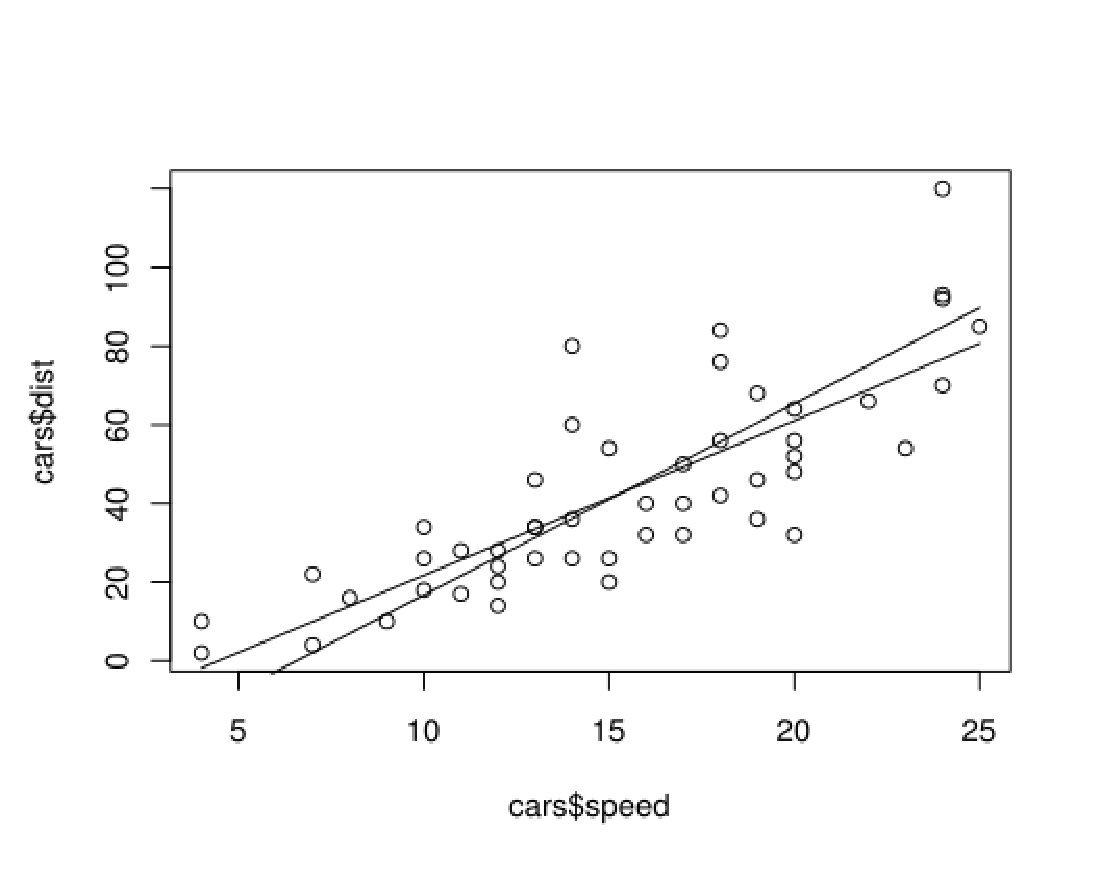
\includegraphics[height=4.2cm,bb=-0 -0 515 350,clip]{CarsRegression.eps}}
\psframe[linewidth=0.02,linecolor=gray](-6.2,-7)(6.2,2.2)
\psframe[linewidth=0.02,linecolor=gray](-6.15,-6.95)(6.15,2.15)
\rput(0,1.4){\color{myblue}\large Math 207:  Introduction to Statistics}
\rput(0,0.6){\color{myblue}Chapter 10:  Regression}
%\psframebox(0,0)(4,4)
\rput(0,-4.4){\scriptsize Dr.~Ralph Wojtowicz}
%\rput(0,-4.9){\scriptsize CME Department}
\rput(0,-5.6){
\includegraphics[height=2cm]{sulogolong.eps}}
%
%\rput(0,-6.5){\scriptsize 6 February 2012}
\end{pspicture}
\end{center}

\end{frame}

%\section[Outline]{}

\addtocounter{page}{-1}
\addtocounter{framenumber}{-1}

{\footnotesize
\frame{\tableofcontents}
}

\section{Regression Line}
\subsection{The Regression Line}
\begin{frame}[t]\frametitle{The Regression Line}
{\small
\begin{itemize}
\item The regression line for $y$ on $x$ estimates the average value for $y$ 
corresponding to each value of $x$.
\item Associated with each increase of one SD in $x$, there is an increase of only $r$ SDs in $y$, on the average.
\item To see why $r$ is the right factor, consider the cases
  $r=0$, $r=1$ and $r=-1$.
\item The regression line is a smoothed version of the graph of averages.
\item The equation for the regression line is: % (where $r=\mbox{the correlation
  %  coefficient}$):
\end{itemize}
%\[(y-\mbox{mean}_y) = r\,\frac{\mbox{SD}_y}{\mbox{SD}_x}\,(x-\mbox{mean}_x)\]

\begin{center}
\begin{pspicture}(-5,0)(4.0,2.5)
  \psset{xunit=0.9,yunit=0.9}
  \rput(-3.5,1.25){$\displaystyle (y-\mbox{mean}_y) = r\,\frac{\mbox{SD}_y}{\mbox{SD}_x}\,(x-\mbox{mean}_x)$}
\psline{->}(0,0)(5,0)
\psline{->}(0,0)(0,3)
\psdot(1,1)
\psline[linewidth=0.02](1,1)(4,1)(4,2.5)
\psline[linewidth=0.02,linecolor=blue](1,1)(4,2.5)
\rput[b](1.4,2.25){\footnotesize $(\mbox{mean}_x, \mbox{mean}_y)$}
   \psline[linewidth=0.02]{->}(1.4,2.2)(1.02,1.1)
\rput[t](2.5,0.9){\footnotesize $\mbox{SD}_x$}
\rput[l](4.1,1.75){\footnotesize $r\,\mbox{SD}_y$}
\end{pspicture}
\end{center}
}
\end{frame}

\section{Example}
\subsection{Example}
\begin{frame}
\frametitle{Example p.\ 165 (part I)}

\footnotesize 

For the men age 18--24 in HANES5, the relationship between height and 
weight can be summarized as follows:\vspace{-3pt}
\begin{center}
{\setlength{\tabcolsep}{2pt}\begin{tabular}{rclcrclcc}
average height & $\approx$ & 70 inches, & \hspace{5pt} & SD & $\approx$ & 3 inches,\\
average weight & $\approx$ & 180 pounds, & \hspace{5pt} & SD & $\approx$ & 45 pounds, &
   \hspace{10pt} $r\approx 0.40$\\[-8pt]
\end{tabular}}
\end{center}
\begin{itemize}
\item<2-> Find the equation for the regression line to predict weight from height.\vspace{-5pt}
  \begin{align*}
  (y - 180) &= 0.4\cdot \frac{45}{3}\,(x - 70)\\[1pt]
{\color{blue}  (y - 180)} &= {\color{blue}6\,(x - 70)}\vspace{-8pt}
\end{align*}
\item<3-> Predict the weight of a subject who was 6'2".\vspace{-5pt}
    \[y = 180 + 6\,(74 - 70) = 180 + 24 = 204\;\mbox{pounds}\vspace{-5pt}\]
\item<4-> Predict the weight of a subject who was 5'6".\vspace{-5pt}
    \[y = 180 + 6\,(66 - 70) = 180 - 24 = 156\;\mbox{pounds}\vspace{-5pt}\]
\item<5-> What was the average weight of all subjects  who were 6'2" tall?\\
    Answer:  same as the previous answer:  204 pounds.
\end{itemize}
\end{frame}

\subsection{Example}
\begin{frame}
\frametitle{Example p.\ 165 (part II)}

\footnotesize 
For the men age 18--24 in HANES5, the relationship between height and 
weight can be summarized as follows:\vspace{-3pt}
\begin{center}
{\setlength{\tabcolsep}{2pt}\begin{tabular}{rclcrclcc}
average height & $\approx$ & 70 inches, & \hspace{5pt} & SD & $\approx$ & 3 inches,\\
average weight & $\approx$ & 180 pounds, & \hspace{5pt} & SD & $\approx$ & 45 pounds, &
   \hspace{10pt} $r\approx 0.40$\\[-8pt]
\end{tabular}}
\end{center}
\begin{itemize}
\item<2-> Find the equation for the regression line to predict {\color{darkgreen}height} from 
   {\color{darkgreen}weight}.\vspace{-5pt}
  \begin{align*}
  (y - 70) &= 0.4\cdot \frac{3}{45}\,(x - 180)\\[1pt]
{\color{blue}  (y - 70)} &= {\color{blue}\frac{2}{75}\,(x - 180)}\vspace{-8pt}
\end{align*}
\item<3-> Predict the height  of a subject who weighed  204 pounds.\vspace{-5pt}
    \[y = 70 + \frac{2}{45}\,(204 - 180) = 70 + 0.64 = 70.64\;\mbox{inches}\vspace{-5pt}\]
\item<4-> Predict the height of a subject who weighed 156 pounds.\vspace{-5pt}
    \[y = 70 + \frac{2}{45}\,(156 - 180) = 70 - 0.64 = 69.36\;\mbox{inches}\vspace{-5pt}\]
\item<5-> What was the average height of all subjects  who weighed 204 pounds?\\
    Answer:  same as the previous answer:  70.64 inches.
\end{itemize}

\end{frame}

\subsection{Using \texttt{R} to Find a Regression Line}
\begin{frame}\frametitle{Using \texttt{R} to Find a Regression Line}
{\scriptsize
\begin{itemize}
\item Example from pages 132--133.\\
   \texttt{> x <- c(1, 3, 4, 5, 7)}\\
   \texttt{> y <- c(5, 9, 7, 1, 13)}\\
   %\texttt{> source("http://www.adjoint-functors.net/SDline.R")}\\
   %\texttt{> SDline(x, y)}\\
   %\texttt{\ \ \ \$meanX=4, \$meanY=7, \$slope=2, \$correlation=0.4}\\[3pt]
   \texttt{> linearModel <- lm(y $\sim$ x)}\\
   \texttt{> summary(linearModel)}\\
   \texttt{Coefficients:}\\
   \texttt{\hphantom{Coefficients}Estimate Std.~Error t value Pr(>|t|)}\\
   \texttt{(Intercept)            \ \  {\color{darkgreen}3.800}\ \ \ \ \ \ 4.733 
             \ \ 0.803 \ \ \   0.481}\\
   \texttt{x\hphantom{(coefficient}    {\color{blue}0.800}\ \ \ \ \ \ 1.058  
             \ \ 0.756 \ \ \   0.505}\\
   \texttt{Residual standard error:  4.733 on 3 degrees of freedom}\\
   \texttt{Multiple R-squared:~0.16, Adjusted R-squared:~-0.12}\\
   \texttt{F-statistic:~0.5714 on 1 and 3 DF, p-value:~0.5046}
\end{itemize}
\begin{center}
\begin{pspicture}(0,0)(7,2.5)
\psset{xunit=1, yunit=0.2}
%\psframe(0,0)(7,3)
\psdots*[linecolor=blue](1,5)(3,9)(4,7)(5,1)(7,13)
\psline[linewidth=0.02](1,4.6)(7,9.4)
\psaxes[Dy=2](0,0)(7,0)(0,13)
\end{pspicture}
\end{center}
}
\end{frame}

\subsection{Plot the SD and Regression Lines}
\begin{frame}\frametitle{Plot the SD and Regression Lines}
{\footnotesize 
\rput(9,-2.2){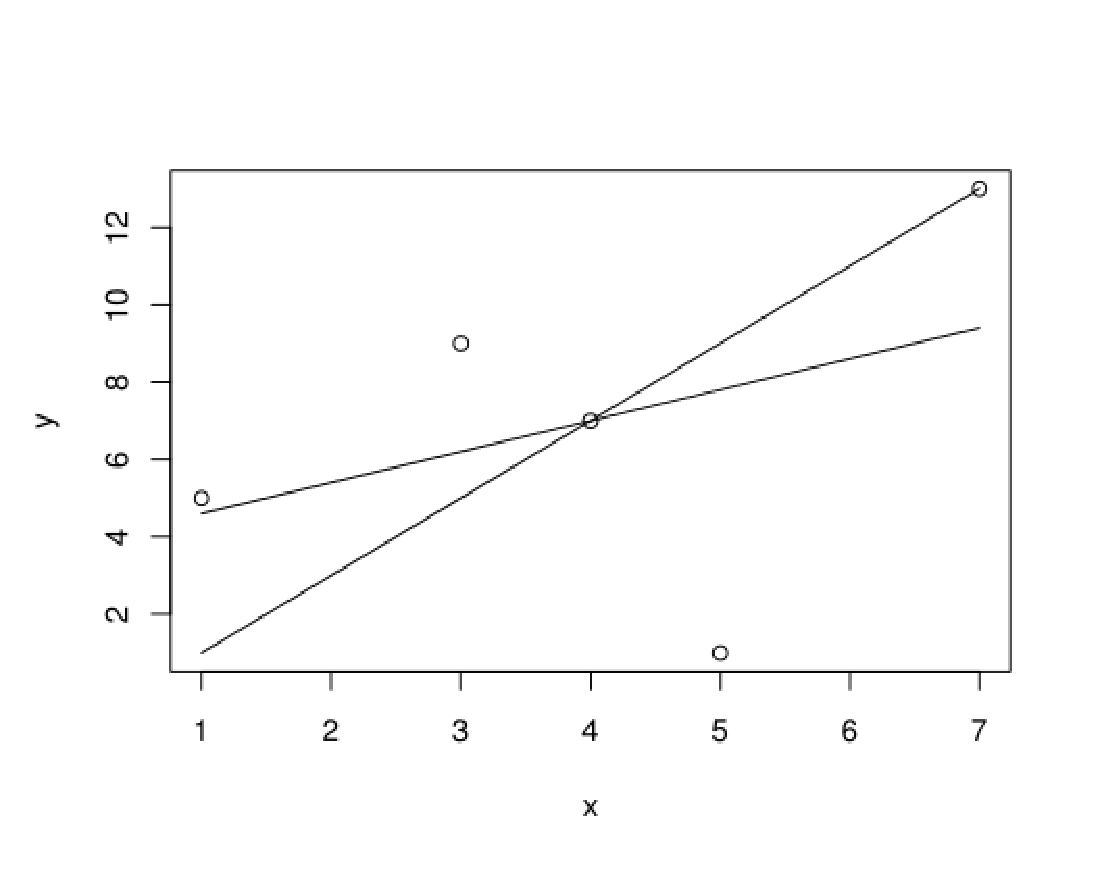
\includegraphics[height=1.8in,bb=-0 -0 515 350,clip]{Regress1.eps}}
\begin{itemize}
\item Example from pages 132--133\\
   \texttt{> x <- c(1, 3, 4, 5, 7)}\\
   \texttt{> y <- c(5, 9, 7, 1, 13)}\\[3pt]
   \texttt{> mean(x)}\\
   \texttt{[1] 4}\\
   \texttt{> mean(y)}\\
   \texttt{[1] 7}\\
   \texttt{> sd(y)/sd(x)}\\
   \texttt{[1] 2}\\[5pt]
 The SD line is $(y-7) = (+1)\cdot 2\,(x - 4)$\\
  \texttt{> cor(x, y)}
   \texttt{[1] 0.4}\\[5pt]
  The regression line is $(y-7)=0.4\cdot 2\,(x - 4)$\\[5pt]
   \texttt{> plot(x, y)}\\
   \texttt{> lines(x, 2*x - 1, type="l")}\\
   \texttt{> lines(x, 0.8*x + 3.8, type="l")}%\vspace{-10pt}
\end{itemize}
}
\end{frame}

\subsection{mtcars Data}
\begin{frame}\frametitle{Cars Data}
{\scriptsize

\begin{itemize}
\item Use the following to get the equation for the regression lines for the mtcars data:\\[3pt]
   \texttt{model = lm(mtcars\$mpg $\sim$  mtcars\$wt)}\\[3pt]
   \texttt{summary(model)}\\[3pt]
   \texttt{plot(mtcars\$wt, mtcars\$mpg, col='blue', xlab='Weight', ylab='MPG')}\\
   \texttt{abline(model)}\vspace{-15pt}
\begin{center}
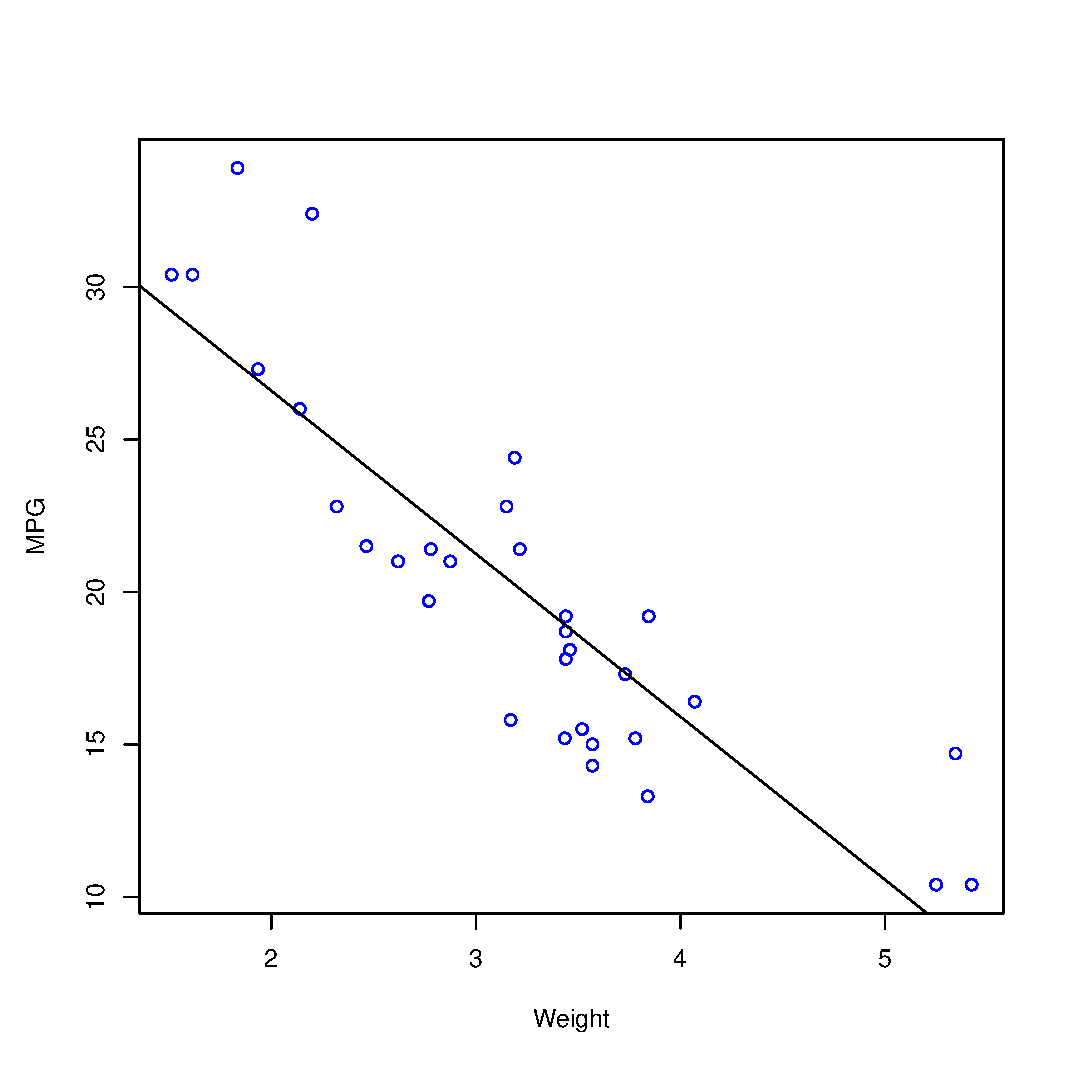
\includegraphics[height=1.5in]{mtcars1.eps}
\end{center}
\item Try some other combinations of variables.
\end{itemize}
}
\label{lastpage}
\end{frame}

\end{document}
